\documentclass[a4paper, 12pt]{article}
\usepackage[left=1.5cm, text={18cm, 25cm}, top=2.5cm]{geometry}
\usepackage[utf8]{inputenc}
\usepackage[czech]{babel}
\usepackage{cite}
\usepackage{graphicx}
\usepackage{float}
\usepackage{amsmath}
\usepackage{tikz}
\usepackage{url}
\usepackage{comment}
\newcommand{\myuv}[1]{\quotedblbase #1\textquotedblleft}
\newcommand{\defVal}[1]{$Default=#1$}

\title{Implementace algoritmu Enumeration sort}
\author{Martin Hruška\\xhrusk16@stud.fit.vutbr.cz}

\date{}
\begin{document}

\maketitle

\section{Úvod}
\label{sec:intro}
Enumeration sort je paralelní řadící algoritmus, který může pracovat s~procesory uspořádanými v~mřížce nebo v~lineárním poli.
Tato práce se zabývá implementací varianty pro lineární pole procesorů, která řadí
posloupnost obsahující $n$ přirozených čísel z~intervalu $<0,255>$ dle jejich velikosti za použití $n+1$ procesorů.
Pro implementaci byla použita knihovna \emph{openMPI}.
V~tomto dokumentu bude algoritmus napřed
stručně popsán a bude provedena teoretická analýza jeho složitosti \ref{sec:analysis},
následně budou popsány implementační detaily \ref{sec:impl},
provedené experimenty \ref{sec:exprmts}
a na závěr je uveden sekvenční diagram znázorňující komunikaci jednotlivých procesorů \ref{sec:seq}.

\section{Popis a analýza algoritmu}
\label{sec:analysis}
Algoritmus zde bude popsán stručně,
ale zároveň dostatečně přesně na to, aby z~tohoto popisu bylo možno dále provést analýzu složitosti algoritmu.
Enumeration sort tedy pracuje následujícím způsobem:
\begin{enumerate}
\item Každý vstupní procesor má registry $X, Y, C, Z$ a registr $C$ na úvod nastaví
na hodnotu jedna.
\item Provádí se cyklus o~$2*n$ opakováních, kde v~prvních $k$ cyklech takových, že $k\leq n$,
je $k$-tý prvek přiřazen $k$-tému procesoru do registru $X$.
Registry $Y$ postupně prochází vstupní posloupnost tak, že v~každém cyklu se posune prvek posloupnosti z~daného procesoru
do jeho následníka v~poli procesorů a do prvního procesoru jsou takto nahrávány prvky vstupní posloupnosti.
Procesory v~každém cyklu porovnají hodnoty v~registru $X$ a $Y$ (pokud mají tyto definovány)
a pokud $X < Y$, tak inkrementují registr $C$ o~jedničku.
V~každém $k$-tém cyklu (kde $k \geq n$) je pak přiřazena hodnota z~registru $X$ $k-n$-tého procesoru do registru $Z$ procesoru,
jenž je v~poli procesorů na stejné pozici jako je daná hodnota v~seřazené posloupnosti.
\item V~závěrečném kroku jsou pak v~cyklu hodnoty z~registru $Z$ přesouvány na výstup tak, že je hodnota
z~registru $Z$ jednoho procesoru přenesena do registru $Z$ procesoru, který ho v~poli procesorů následuje.
Z~posledního procesoru v~poli je pak přenesena tato hodnota na výstup.
\end{enumerate}

Nyní přistupme k~analýze časové složitosti algoritmu.
První bod z~popisu algoritmu, tedy inicializace registru $C$ na hodnotu jedna je možno provést v~konstantním čase,
zapsáno v~$O$ notaci jako $O(1)$.
V~druhém bodě se proveden cyklus $2*n$-krát a každý krok cyklu lze provést v~konstantním počtu kroků, dohromady tedy
má složitost $2*n*c=O(n)$, kde $c$ je konstanta udávající počet kroků výpočtu v~těle cyklu.
Třetí bod je cyklus s~$n$ opakováními a každý cyklu lze provést také v~konstantním počtu kroků, celkem pak $n*c_2=O(n)$,
kde $c$ je konstanta udávající počet kroků výpočtu v~těle cyklu.
Celý výpočet má tedy časovou složitost $t(n)=O(1)+O(n)+O(n)=O(n)$.
Počet procesorů nutných k~výpočtu je $n$, a tedy $p(n)=n$.
Cena paralelního řešení $c(n)$ je $p(n)*t(n)=n*O(n)=O(n^2)$.


\section{Implementace}
\label{sec:impl}
Při samotné implementaci byl respektován algoritmus tak, jak by popsán předchozí části \ref{sec:analysis}, až na změny či upřesnění popsané v~této části.

Vstupní posloupnost čísel program načítá ze souboru \emph{numbers}, kde je uložena jako sekvence bytů.
Proto existovaly dvě možnosti implementace samotného algoritmu.
V~první by probíhalo samotné načítání hodnot ze souboru během cyklu algoritmu prvním (master) procesorem.
Tento přístup by ale byl nevhodný pro další měření rychlosti algoritmu, protože ta by byla
zkreslena režií spojenou s~načítáním dat ze souboru a průběžným zasíláním zpráv s~aktuálním počtem hodnot
ve vstupní posloupnosti ostatním procesorům.
Toto bylo potvrzeno implementací a experimenty.
Proto byla implementace provedena druhým způsobem, při němž první procesor načte všechny prvky posloupnosti,
informuje o~jejich počtu ostatní procesory a při samotném řazení posloupnosti jsou pak hodnoty čteny přímo z~paměti.

Samotný algoritmu Enumeration sort byl upraven tak, aby byl schopen řadit posloupnosti i se stejnými čísly.
Toho bylo dosaženo tak, že v~druhém kroku algoritmu (viz. sekce \ref{sec:analysis}) není provedeno
porovnání $X<Y$, ale $X \leq Y$ pro všechna čísla, která jsem ve vstupní posloupnosti na pozici s~pořadovým
číslem větším, než je pořadové číslo procesoru v~poli procesorů.

\section{Experimenty}
\label{sec:exprmts}

\begin{figure}[bt]
\begin{center}
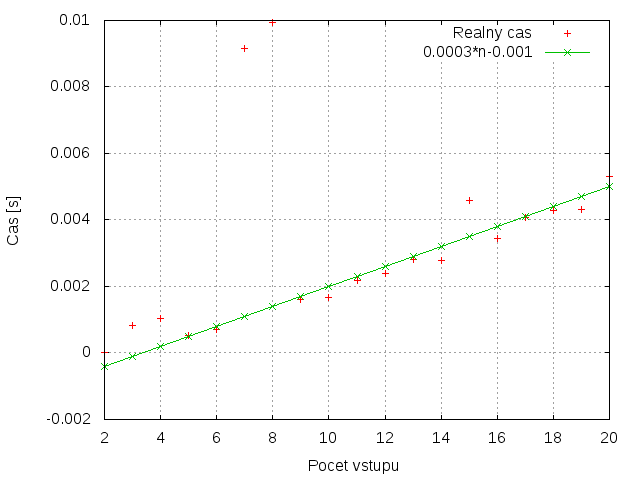
\includegraphics[scale=0.8]{plots/perf.png}
\caption{Doba v~sekundách nutná pro seřazení posloupnosti v~závislosti na její délce.}
\end{center}
\end{figure}
\label{fig:exp}

S~vytvořeným programem byly následně provedeny experimenty s~posloupnostmi o~různé délce, tak aby bylo
možné porovnání s~teoreticky odvozenou složitostí výpočtu.
Experimenty byly provedeny na počítači \emph{merlin.fit.vutbr.cz} a čas byl měřen pomocí
funkce $MPI:Wtime$, která byla volána napřed samotným začátkem řazení (tedy až po načtení vstupní posloupnosti ze souboru)
a poté po seřazení a uložení výsledku do výstupní posloupnosti.
Obě hodnoty byly od sebe následně odečteny a tím byla získána doba řazení.
Délka posloupnosti byla dle doporučení z~předchozího projektu omezena na $20$ prvků, jelikož při
větší délce nebyly výsledky kvůli systémovým omezením relevantní.
%Experiment byl proveden s~vědomím omezené relevance výsledků při měření výkonů na takto malé vzorku dat.
Provedené měření lze vidět na obrázku \ref{fig:exp}.
Na grafu červené body udávají reálnou dobu v~sekundách, kterou program potřeboval pro seřazení
posloupnosti o~zadaném počtu prvků.
Zeleně je pak přímka znázorňující funkci $0.0003*n-0.001$, která ilustruje
časovou složitost $O(n)$, jež by měl mít algoritmus teoreticky.
Z~grafu je patrné, že časová náročnost implementace se také drží v~lineárním čase,
a tudíž byl potvrzen teoretický odhad časové složitosti.

\section{Sekvenční diagram}
\label{sec:seq}
Na sekvenčním diagramu na obrázku \ref{fig:seq} je znázorněna komunikace mezi procesory.
Proměnné $i,j$ udávají pořadové číslo procesoru v~poli procesorů,
procesor $0$ je na prvním místě v~poli procesorů
a \emph{ostatní} představuje všechny procesory kromě i-tého procesoru.
Pole procesorů použitých pro řazení je indexováno od nuly.
\begin{figure}
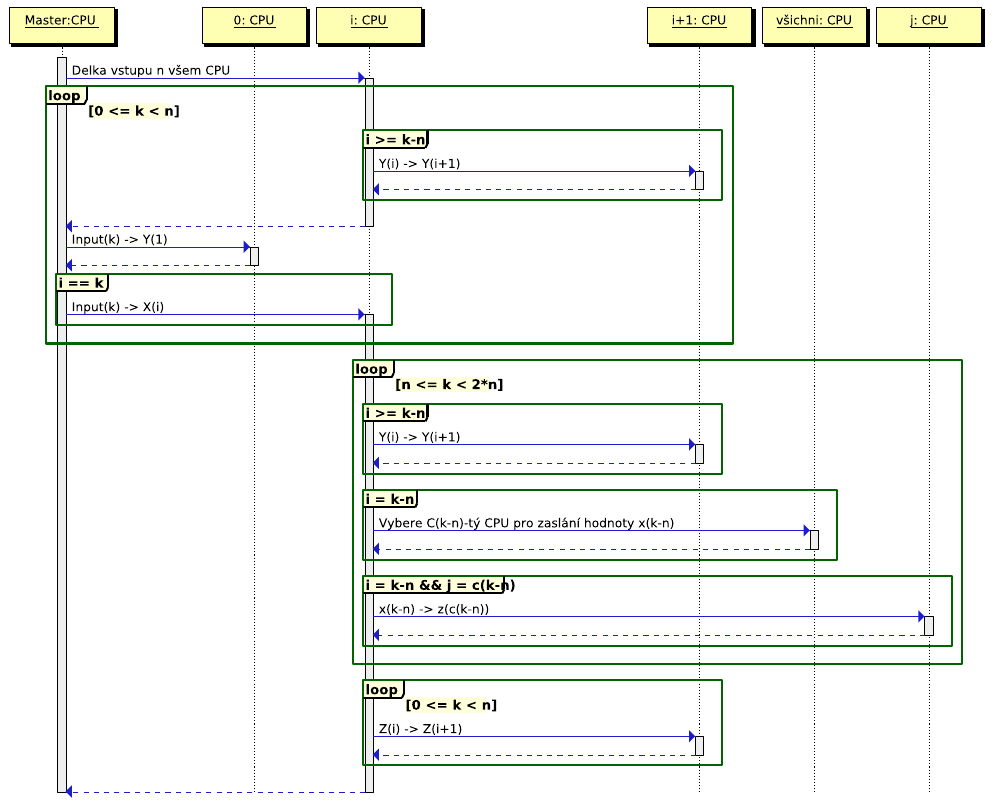
\includegraphics[scale=0.7]{seq.png}
\caption{Sekvenční diagram znázorňující komunikaci mezi procesory}
\end{figure}
\label{fig:seq}

\section{Závěr}
Byl implementován algoritmus Enumeration sort s~lineárním polem procesorů a s~touto implementací byly provedeny
experimenty s~měřenín časové náročnosti výpočtu. Ta byla poté porovnána s~teoreticky odvozenou časovou složitostí a
bylo zjištěno, že rychlost implementace odpovídá teoretické analýze složitosti.
V~práci je také uveden sekvenční diagram popisující komunikační protokol implementovaného algoritmu.

\end{document}
